\chapter{Założenia projektowe}
\section{Eksploracja danych}
Eksploracja danych (ang. data mining) jest dziedziną nauki zajmującą się metodami pozyskiwania wiedzy z danych. Główne metody eksploracji danych to klasteryzacja i klasyfikacja danych, odkrywania wzorców asocjacji lub sekwencji, selekcja danych odstających. Algorytmy wykorzystywane do eksploracji danych pochodzą głównie z zakresu statystyki i uczenia maszynowego \cite{9783319141411}. Zwykle, aby wydobyć wiedzę np. z tekstu, musimy przetworzyć ogromne ilości danych. Źródłem tych danych mogą być strony WWW, artykuły w gazetach czy wiadomości E-mail. Dzięki eksploracji można wydobyć kolejno: informacje o konkretnym produkcie ze strony WWW, określić treść dokumentów tekstowych oraz określić czy dany E-mail jest spamem. 

\subsection{Klasteryzacja}
Klasteryzacja (grupowanie) inaczej nazywana jest klasyfikacją bez nadzoru. To metoda, dzięki której następuje pogrupowanie pewnego zbioru elementów w taki sposób, aby dane poszczególnych grup były do siebie jak najbardziej podobne. Grupowanie dąży do tego, aby odległości pomiędzy obiektami w jednej grupie były jak najmniejsze, natomiast odległość pomiędzy grupami obiektów - jak największa.

Na wykresie \figurename{\ref{fig:threeblobs}} osadzone są pewne obiekty. Trzema różnymi kolorami oznaczono przynależność do grupy. Możemy zaobserwować, że obiekty należące do tej samej grupy są skupione wokół siebie.

\begin{figure}[h!]
    \centering
    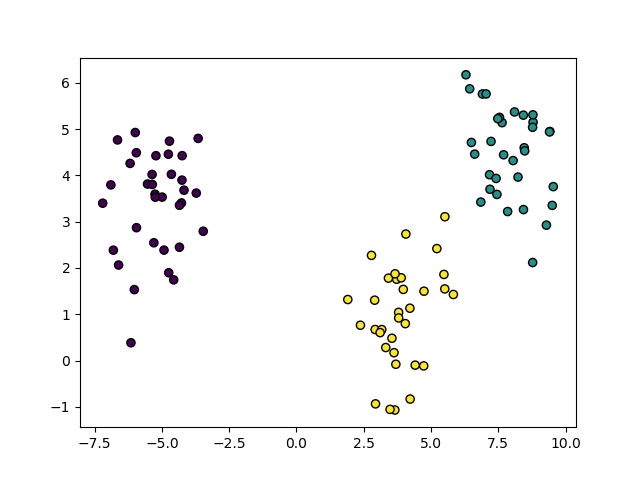
\includegraphics[scale=0.5]{Rysunki/Rozdzial2/4.png}
    \caption{Pogrupowane obiekty}
    \label{fig:threeblobs}
\end{figure}

\section{Python}
Python jest wieloplatformowym językiem programowania wysokiego poziomu. Został stworzony w celu zapewnienia dużej czytelności kodu źródłowego. Składnia tego języka jest przejrzysta dzięki zminimalizowaniu konstrukcji składniowych. Korzysta on z wcięć zamiast klamr, które oznaczają początek i koniec bloku instrukcji. Python rozwijany jest jako otwarty projekt (ang. open-source). Instalacja Pythona sprowadza się do pobrania instalatora oraz uruchomienia go, pamiętając, aby podczas instalacji zaznaczyć zgodę na dodanie przez instalator ścieżki Pythona do zmiennych środowiskowych systemu. Do realizacji niniejszej pracy wykorzystano Pythona w wersji 3.6.4.

%\begin{figure}[h!]
%  \centering
%  \subfloat{\label{fig:checkboxPython}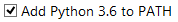
\includegraphics[width=0.40\textwidth]{Rysunki/Rozdzial2/1.png}}
%  \caption{Wymagane pole do zaznaczenia podczas instalacji oprogramowania}
%  \label{fig:srodowiskoPracyPy}
%\end{figure}

Weryfikacja poprawności instalacji języka programowania sprowadza się do uruchomienia programu z wiersza poleceń systemu Windows. Wówczas uruchamiamy program Python, w którym już teraz jest możliwość pisania mało skomplikowanych programów.

\begin{figure}[h!]
    \centering
    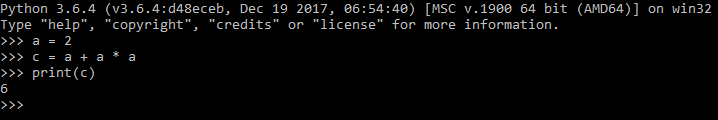
\includegraphics[scale=0.7]{Rysunki/Rozdzial2/5.png}
    \caption{Prosty przykład programu napisanego w języku Python w wierszu poleceń}
    \label{fig:simplePythonCmd}
\end{figure}

\section{Środowisko pracy}
Projekt powstał w środowisku Visual Studio Code w wersji 1.19.2 od firmy Microsoft oraz został napisany w języku Python w wersji 3.6.4. Środowisko to dostępne jest na platformach między innymi Windows, Linux i macOS. Środowisko jest darmowe oraz open-source.


Instalacja środowiska programistycznego na platformie Windows przebiega w bardzo prosty sposób. 
Pierwszym etapem jest instalacja Visual Studio Code, czyli edytora kodu, który wspiera najważniejsze operacje programowania. Tymi operacjami są na przykład debugowanie czy system kontroli wersji. Środowisko to zostało stworzone z myślą o szybkich cyklach pisania kodu oraz debugowania. Podczas instalacji należy zaznaczyć pole, które doda ścieżkę oprogramowania do zmiennych środowiskowych systemu operacyjnego.
\begin{figure}[h!]
  \centering
  \subfloat{\label{fig:checkboxVSC}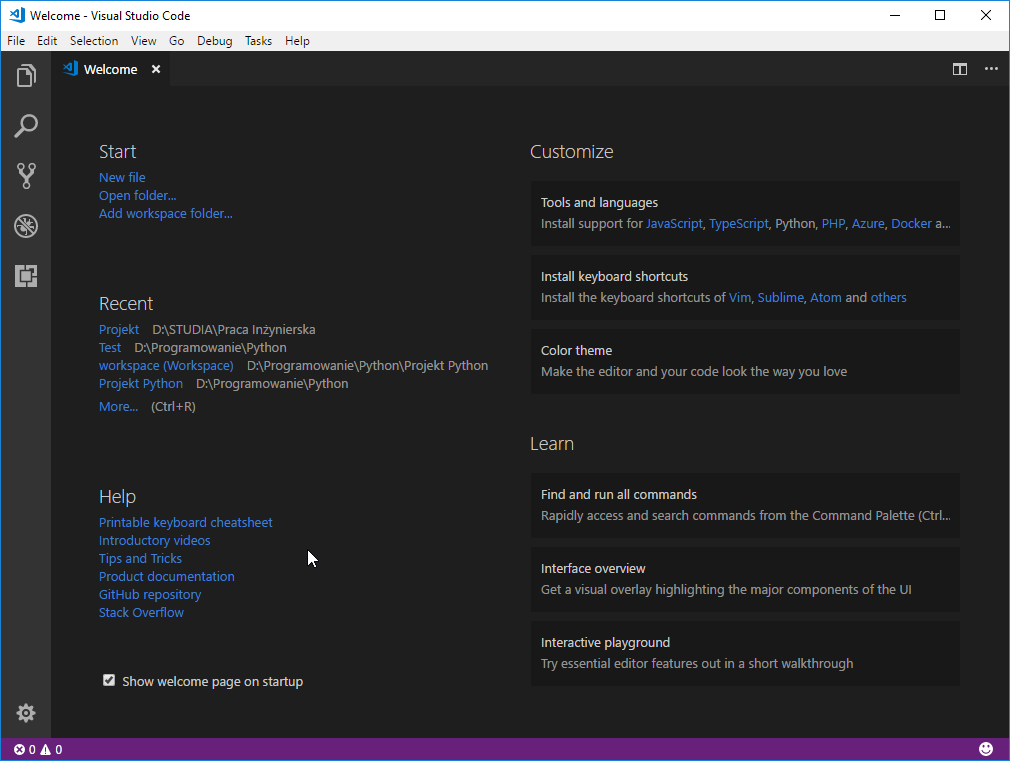
\includegraphics[width=0.9\textwidth]{Rysunki/Rozdzial2/srodowisko.png}}
  \caption{Interfejs środowiska Visual Studio Code}
  \label{fig:srodowiskoPracyVs}
\end{figure}

Kolejnym etapem jest konfiguracja wykorzystywanego środowiska, by móc uruchomić pisane w języku Python programy. W tym celu należy utworzyć nowy folder, który jest odpowiednikiem projektu w innych środowiskach programowania. Następnie stworzyć plik o rozszerzeniu \textit{.py}. W tym momencie pojawi się komunikat o zainstalowaniu rozszerzenia do Visual Studio Code, z dodatkami do języka Python, takimi jak:
\begin{itemize}
    \item formatowanie kodu,
    \item refaktoryzacja,
    \item pilnowanie składni języka,
    \item podpowiedzi.
\end{itemize}
Należy go zainstalować oraz zresetować Visual Studio Code klikając przycisk "Reload" obok dodanego rozszerzenia.


Następnie wchodzimy w zakładkę "Debug (Ctrl+Shift+D)" i klikamy na rozwijaną listę, po czym wybieramy opcję "Add Configuration...". W tym miejscu na górze programu wyświetlą się propozycje zainstalowanych w systemie środowisk. Po dodaniu konfiguracji Python, utworzy nowy folder o nazwie ".vscode" oraz plik "launch.json", w którym są wszystkie konfiguracje programu. Najważniejszą konfiguracją ze wszystkich jest ta położona na samej górze z nazwą "Python", ponieważ bez niej nie będziemy w stanie uruchamiać programów. Ostatnim elementem konfiguracji jest dodanie ścieżki dostępu do języka programowania. W zakładce "Explorer (Ctrl+Shift+E)" należy kliknąć prawym przyciskiem myszy i wybrać "Open Folder Settings". Utworzy się nowy plik w folderze ".vscode" o nazwie "settings.json", w którym są wszelkie opcje projektu. Po uruchomieniu tego pliku klikamy po prawej stronie "Workspace Settings", gdzie podajemy ścieżkę do programu Python.

\begin{figure}[h!]
    \centering
    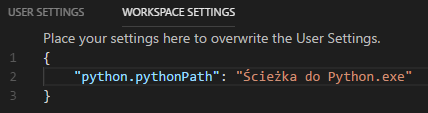
\includegraphics{Rysunki/Rozdzial2/3.png}
    \caption{Absolutna ścieżka do zainstalowanego programu Python.exe}
    \label{fig:pythonPath}
\end{figure}

Ostatnim krokiem jest weryfikacja, czy wszystko zostało poprawnie skonfigurowane. W tym celu wystarczy otworzyć stworzony wcześniej plik z rozszerzeniem \textit{.py} i napisać pierwsze standardowe polecenie "print('Hello World!')".

\newpage
\section{Biblioteki do wstępnego przetwarzania dokumentów tekstowych}
Aby zrealizować zaplanowane zadanie klasteryzacji dokumentów konieczne jest wstępne przetworzenie dokumentów tekstowych do postaci akceptowalnej przez procedury klasteryzacji. Język Python oferuje szereg bibliotek, które wspomagają realizację tych procesów. Najczęściej wykorzystywane do takich zadań biblioteki to Scikit-learn \cite{scikit-learn} oraz Natural Language Toolkit \cite{Loper02nltk:the}.

\subsection{Scikit-learn}
Scikit-learn jest darmową biblioteką do wykonywania czynności związanych z uczeniem maszynowym. Wprowadza wiele rozwiązań, jak: algorytmy klasyfikacji, regresji czy klasteryzacji. 

Biblioteka wymaga dodatkowo kilka innych modułów by działać poprawnie. Tymi modułami są:
\begin{itemize}
    \item NumPy w wersji wyższej bądź równej 1.8.2
    \item SciPy w wersji wyższej bądź równej 0.13.3
\end{itemize}

Instalacja bibliotek odbywa się z wiersza poleceń. Istnieją dwa sposoby realizacji tej procedury. Pierwszy z nich polega na uruchomieniu wiersza poleceń z samego Windowsa. W drugim instalacja odbywa się poprzez Terminal w Visual Studio Code, który ma wbudowaną w sobie integrację z Windows PowerShell. Jest to odpowiednik wiersza poleceń.

Kolejnym etapem jest instalacja wymaganych modułów dla języka Python. Instalację można przeprowadzić z wykorzystaniem menadżera pakietów "pip" wydając następujące polecenia: "pip install {nazwa modułu}", dla wyżej wymienionych bibliotek:
\lstinputlisting[label={lst:2},caption={Instalacja wymaganych modułów z podaniem wersji}, language=python, showstringspaces=false]{Algorytmy/Rozdzial2/pipInstall.py}

Aby zainstalować najnowsze wersje tych bibliotek
\lstinputlisting[label={lst:3},caption={Instalacja wymaganych modułów z najnowszej wersji}, language=python, showstringspaces=false]{Algorytmy/Rozdzial2/pipInstallNewest.py}

\subsection{Natural Language Toolkit}
NLTK jest narzędziem wspomagającym pisanie programów do przetwarzania języka naturalnego. Biblioteka dostarcza wiele istotnych dodatków, takich jak klasyfikacja, tokenizacja czy stemming (szczegółowy opis tych operacji zaprezentowane w podpunkcie \ref{prepareDocs}).

NLTK jest projektem otwartym (ang. open-source). Jego instalacja przebiega w taki sam sposób co instalacja Scikit-learn. Należy uruchomić wiersz poleceń lub Terminal i wykorzystać do tego programu "pip".
\lstinputlisting[label={lst:4},caption={Instalacja biblioteki NLTK z najnowszej wersji}, language=python, showstringspaces=false]{Algorytmy/Rozdzial2/pipInstallNLTK.py}

Przetestowanie instalacji tej biblioteki należy wykonać poprzez uruchomienie programu "python" z wiersza poleceń lub Terminala w środowisku Visual Studio Code, po czym uruchomić polecenia (\ref{lst:5})
\lstinputlisting[label={lst:5},caption={Weryfikacja poprawności instalacji biblioteki NLTK}, language=python, showstringspaces=false]{Algorytmy/Rozdzial2/importnltk.py}

Wywołanie metody "download()" z pakietu "nltk" spowoduje pojawienie się menadżera ze wszystkimi dodatkami tej biblioteki, "NLTK Downloader", dzięki któremu w łatwy sposób można zainstalować potrzebne dodatki.
\begin{figure}[h!]
    \centering
    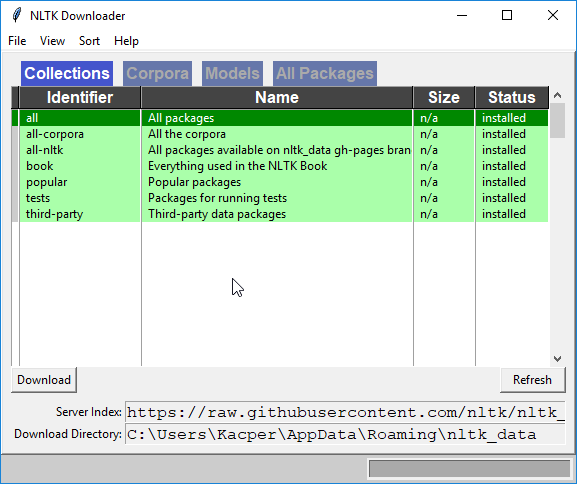
\includegraphics[scale=0.7]{Rysunki/Rozdzial2/6.png}
    \caption{NLTK Downloader}
    \label{fig:nltkdownloader}
\end{figure}

\section{Przygotowanie dokumentów tekstowych} \label{prepareDocs}
Zbyt duża różnorodność w dokumentach tekstowych może sprawić więcej problemów niż początkowo sądzimy. Długie oraz zbędne słowa czy znaki są powszechne niemal w każdych dokumentach tekstowych. Dlatego niezbędne jest wstępne przetworzenie tekstu na potrzeby klasteryzacji, tak by działała jak najkorzystniej. Przygotowywanie dokumentów można podzielić na kilka etapów, które przedstawiono w kolejnych podpunktach.

    \subsection{Tokenizacja} \label{sec:tokenizacja}
    Tokenizacja jest to transformacja dokumentu tekstowego w taki sposób, aby rozdzielić go na pojedyncze słowa. Zazwyczaj w tym momencie używana jest tokenizacja po białych znakach (ang. whitespace). Na zadanym dokumencie tekstowym jest wykonywana operacja dzielenia tekstu w miejscach spacji, nowych linii czy tabulatorów.
    
    Uruchomienie skryptu z listingu \ref{lst:6} podzieli nasz tekst w długą listę słów oraz wypisze 100 pierwszych.
    \lstinputlisting[label={lst:6},caption={Dzielenie tekstu po białych znakach}, language=python, showstringspaces=false, breaklines=true]{Algorytmy/Rozdzial2/splitByWS.py}
    
    Drugi sposób na podzielenie tekstu na części, to skorzystanie z wcześniej omówionej biblioteki Natural Language Toolkit. Biblioteka ta udostępnia gotową metodę do tokenizacji dokumentów tekstowych.
    
    \lstinputlisting[label={lst:7},caption={Dzielenie tekstu z wykorzystaniem biblioteki NLTK}, language=python, showstringspaces=false, breaklines=true]{Algorytmy/Rozdzial2/splitByNLTK.py}
    
    
    Różnice pomiędzy dwoma sposobami tokenizacji są niewielkie. 
    O ile pierwszy sposób rozróżnił słowa po znakach białych, to drugi rozdzielił je dodatkowo od znaków interpunkcyjnych.
    
    
    \subsection{Czyszczenie} \label{sec:czyszczenie}
    Czyszczenie dokumentów tekstowych polega na usunięciu niepotrzebnych elementów dokumentu tekstowego. Takimi elementami są: znaki interpunkcyjne, liczby i wyrazy znajdujące się na stop liście (ang. stopwords). 
    
    Python dostarcza nam gotową listę znaków interpunkcyjnych.
    \lstinputlisting[label={lst:8},caption={Lista wszystkich znaków interpunkcyjnych}, language=python, showstringspaces=false, breaklines=true]{Algorytmy/Rozdzial2/punctuation.py}
    
    Dzięki temu jesteśmy w stanie w łatwy sposób usunąć z tekstu wszystkie znaki interpunkcyjne. Python posiada również wbudowaną metodę "isalpha()", która zwraca wartość prawdziwą tylko wtedy, kiedy wszystkie znaki w tekście należą do zbioru znaków alfanumerycznych.
    
    \lstinputlisting[label={lst:9},caption={Czyszczenie dokumentu tekstowego wykorzystując tokeny z \ref{lst:7}}, language=python, showstringspaces=false, breaklines=true]{Algorytmy/Rozdzial2/cleaning.py}    
    Czyszczenie dokumentu tekstowego z elementów znajdujących się na stop liście (ang. stopwords), również można wykonać za pomocą biblioteki NLTK. Dostarcza ona predefiniowane stop listy w różnych językach. 
    \newpage
    \lstinputlisting[label={lst:10},caption={Kasowanie słów zawartych na stop liście}, language=python, showstringspaces=false, breaklines=true]{Algorytmy/Rozdzial2/stopwords.py}
    
    Istnieje również możliwość wygenerowania własnej stop listy na podstawie analizowanych dokumentów tekstowych. Zwykle taką listę generuje się zliczając ilość unikalnych słów we wszystkich dokumentach tekstowych, a następnie uznając te najbardziej popularne za słowa, które nie są istotne do klasyfikacji dokumentów. Ważnym elementem w tym procesie, jest wyznaczenie progu ilości wystąpień słowa, od którego zależy czy jest ono istotne czy nie.
    
    \subsection{Normalizacja} \label{sec:normalizacja}
    Normalizację (ang. normalization) konkretnych słów w dokumencie tekstowym można wykonać na wiele różnych sposobów. Zwykle polega ona na przyjęciu pewnego wzorca normalizacji dla całego dokumentu i zastosowaniu go do wszystkich słów w tekście. Jedną z metod normalizacji jest zwykła zamiana wszystkich słów w dokumencie na słowa z małymi literami (ang. lowercase) \cite{normalizeText}. Kolejnym krokiem jest normalizacja dat. Zapis dat w różnych częściach świata jest różny \cite{wiki:Date_format_by_country}. Jednak każdy miesiąc posiada swój unikalny skrót \cite{skrotyMiesiecy}, który należałoby znormalizować, czyli zamienić na pełne nazwy miesięcy. 
    
    Ostatnim etapem normalizacji jest stemming. Pierwsze próby zastosowania algorytmu stemmingu zostały zaproponowane w latach 60. XX wieku. Słowa o takim samym znaczeniu, które zapisane są na kilka różnych sposobów mogą być poddane stemmingowi. Proces ten kasuje końcówki fleksyjne ze słów w dokumencie tekstowym pozostawiając tylko część słowa zwaną rdzeniem. Można wyróżnić kilka rodzajów algorytmów stemmingu:
    \begin{itemize}
        \item Lancaster Stemmer,
        \item Snowball Stemmer,
        \item Porter Stemmer.
    \end{itemize}
    
    \lstinputlisting[label={lst:11},caption={Zastosowanie powyższych rodzajów stemmingu}, language=python, showstringspaces=false, breaklines=true]{Algorytmy/Rozdzial2/stemming.py}
    \newpage
    \subsection{TF-IDF} \label{sec:tfidf}
        Ważnym elementem grupowania dokumentów tekstowych, jest dobór odpowiednich cech opisujących dokument. Cechy ekstrachowane są z dokumentów tekstowych w ten sposób, aby dokumenty o podobnej treści uzyskiwały podobne wektory wartości cech. Dokumenty tekstowe o treściach różniących się od siebie powinny zostać opisane różnymi wektorami wartości cech.
        
        $TF-IDF$ (ang. TF - term frequency, IDF - inverse document frequency) jest klasyczną metodą, dzięki której możliwe jest przypisywanie wag poszczególnym słowom kluczowym opisującym dokument tekstowy.
        \begin{equation}
            \begin{bmatrix}
            $$w_{d_1t_1}$$ & . & . & $$w_{d_nt_1}$$\\ 
            . & . &  & .\\ 
            . &  & . & .\\ 
            $$w_{d_1t_n}$$ & . & . & $$w_{d_nt_n}$$
            \end{bmatrix}
        \end{equation}
        gdzie $w_{d_1t_1}$ to obliczona waga słowa $t_1$ w dokumencie $d_1$.
        
        
        Aby wyznaczyć wagi dla dokumentu tekstowego i policzyć współczynnik $TF-IDF$ należy w pierwszej kolejności obliczyć miary:
        \begin{itemize}
            \item częstotliwości występowania wyrażeń (ang. term frequency - $TF$) - $TF(t_i, d)$ - liczba wystąpień słowa $t_i$ w dokumencie d,
            \item częstotliwości dokumentów (ang. document frequency) - $DF(t_i)$ - liczba dokumentów tekstowych, w których istnieje słowo $t_i$,
            \item odwrotnej częstości dokumentu (ang. inverse document frequency - $IDF$) - $IDF(t_i) = 1+\ln{\left(\frac{|D|}{DF(t_i)}\right)}$ \cite{tfidf} gdzie |D| to liczba wszystkich dokumentów tekstowych,
        \end{itemize}
        $TF-IDF$ jest iloczynem miar $TF$ oraz $IDF$. 
        Przykładowo dla podanych poniżej trzech dokumentów tekstowych:
        \begin{itemize}
            \item $d1$ = The game of life is a game of everlasting learning,
            \item $d2$ = The unexamined life is not worth living,
            \item $d3$ = Never stop learning
        \end{itemize} należy na samym początku policzyć "term frequency", czyli ilość występowania danego słowa w dokumencie tekstowym. Drugą istotną rzeczą w tym etapie jest znormalizowanie $TF$. Normalizacja odbywa się za pomocą wzoru:
        \begin{equation}
            NTF(t_i, d) = \frac{TF(t_i, d)}{|C_d|}
        \end{equation}
        gdzie $|C_d|$ to ilość słów w dokumencie tekstowym.
        
        
        \begin{table}[h!]
            \centering
            \caption{Obliczone wartości $TF(t_i, d1)$ i $NTF(t_i, d1)$}
            \label{tfd1}
            \begin{tabular}{|l|l|l|l|l|l|l|l|l|}
            \hline
            $d1$ & the & game & of & life & is & a & everlasting & learning \\ \hline
            $TF(t_i, d1)$        & 1   & 2    & 2  & 1    & 1  & 1 & 1           & 1        \\ \hline
            $NTF(t_i, d1)$ & 0.1 & 0.2 & 0.2 & 0.1 & 0.1 & 0.1 & 0.1 & 0.1 \\ \hline
            \end{tabular}
        \end{table}
        
        \begin{table}[h!]
            \centering
            \caption{Obliczone wartości $TF(t_i, d2)$ i $NTF(t_i, d2)$}
            \label{tfd2}
            \begin{tabular}{|l|l|l|l|l|l|l|l|}
            \hline
            $d2$            & the & unexamined & life & is & not & worth & living \\ \hline
            $TF(t_i, d2)$ & 1   & 1          & 1    & 1  & 1   & 1     & 1      \\ \hline
            $NTF(t_i, d2)$ & 0.1428 & 0.1428 & 0.1428 & 0.1428 & 0.1428 & 0.1428 & 0.1428 \\ \hline
            \end{tabular}
        \end{table}

        \begin{table}[h!]
            \centering
            \caption{Obliczone wartości $TF(t_i, d3)$ i $NTF(t_i, d3)$}
            \label{tfd3}
            \begin{tabular}{|l|l|l|l|}
            \hline
            $d3$            & never & stop & learning \\ \hline
            $TF(t_i, d3)$ & 1     & 1    & 1        \\ \hline
            $NTF(t_i, d3)$ & 0.3333 & 0.3333 & 0.3333  \\ \hline
            \end{tabular}
        \end{table}
        \newpage
        Kolejnym krokiem jest policzenie współczynnika $IDF$ dla każdego termu ze wszystkich dokumentów tekstowych. Ilość wszystkich dokumentów jest równa 3, stąd
        \begin{equation}
            |D| = 3
        \end{equation}
        
        Korzystając ze wzoru
        \begin{equation}
            IDF(t_i) = 1+\ln{\left(\frac{|D|}{DF(t_i)}\right)}
        \end{equation}
        \begin{table}[h!]
            \centering
            \caption{Wartości współczynnika IDF dla wszystkich termów}
            \label{idf}
            \begin{tabular}{|l|l|}
            \hline
            Termy       & $IDF$     \\ \hline
            the         & 1.40546 \\ \hline
            game        & 2.09861 \\ \hline
            of          & 2.09861 \\ \hline
            life        & 1.40546 \\ \hline
            is          & 1.40546 \\ \hline
            a           & 2.09861 \\ \hline
            everlasting & 2.09861 \\ \hline
            learning    & 1.40546 \\ \hline
            unexamined  & 2.09861 \\ \hline
            not         & 2.09861 \\ \hline
            worth       & 2.09861 \\ \hline
            living      & 2.09861 \\ \hline
            never       & 2.09861 \\ \hline
            stop        & 2.09861 \\ \hline
            \end{tabular}
        \end{table}
        
        Ostatnim krokiem jest policzenie dla wszystkich termów współczynników $TF-IDF$. Można zauważyć, że czym większa obliczona waga, tym większa istotność danego słowa w dokumencie, dlatego też uważa się, że termy, które mają największą wagę w danym dokumencie tekstowym, są tymi cechami, które dosyć dobrze opisują jego tematykę. Zaletą współczynnika $TF-IDF$ jest to, że przy odróżnianiu jednego dokumentu tekstowego od innych, wpływ ma nie tylko częstość występowania w nim danego słowa, ale też występowanie tego słowa w innych dokumentach. 
        \begin{table}[h!]
            \centering
            \caption{Wartości współczynnika $TF-IDF$ dla dokumentów tekstowych}
            \label{tfidf}
            \begin{tabular}{|l|l|l|l|}
            \hline
            Termy       & $d1$       & $d2$       & $d3$       \\ \hline
            the         & 0.140546 & 0.200699 & 0        \\ \hline
            game        & 0.419722 & 0        & 0        \\ \hline
            of          & 0.419722 & 0        & 0        \\ \hline
            life        & 0.140546 & 0.200699 & 0        \\ \hline
            is          & 0.140546 & 0.200699 & 0        \\ \hline
            a           & 0.209861 & 0        & 0        \\ \hline
            everlasting & 0.209861 & 0        & 0        \\ \hline
            learning    & 0.140546 & 0        & 0.468439 \\ \hline
            unexamined  & 0        & 0.299681 & 0        \\ \hline
            not         & 0        & 0.299681 & 0        \\ \hline
            worth       & 0        & 0.299681 & 0        \\ \hline
            living      & 0        & 0.299681 & 0        \\ \hline
            never       & 0        & 0        & 0.699466 \\ \hline
            stop        & 0        & 0        & 0.699466 \\ \hline
            \end{tabular}
        \end{table}
        
        \newpage
        Policzenie $TF-IDF$ za pomocą Pythona sprowadza się do wykorzystania biblioteki Scikit-learn posiadającej w sobie klasę TfidfVectorizer, która na wejściu otrzymuje listę dokumentów, a następnie zwraca wszystkie wagi słów. Klasa ta posiada również dużo parametrów, jak "stopwords='english'", która wyklucza wszystkie słowa zawierające się na stop liście.
        
        \lstinputlisting[label={lst:12},caption={Przykład kodu wykorzystanego do policzenia $TF-IDF$ dla dokumentów tekstowych}, language=python, showstringspaces=false, breaklines=true]{Algorytmy/Rozdzial2/tfidf.py}
        \newpage
        
\section{Klasteryzacja danych}
    \subsection{Algorytm k-means} \label{sec:kmeans}
    Algorytm k-Means jest wykorzystywany do partycjonowania danych obserwacyjnych w predefiniowaną ilość klastrów. Algorytm opracowany przez J MacQueen-a (patrz \cite{macqueen1967}) rozpoczyna się od losowego rozmieszczenia zestawu środków klastrów ($\mu$) uważanych za środki klastrów. Podczas każdego kroku aktualizacji wszystkie obserwacje $x$ są przypisywane do najbliższego punktu środkowego (patrz równanie \ref{eqn:kmeansKrok}). W standardowym algorytmie każda obserwacja $x$ (punkt z danymi) jest przypisana do jednego klastra. Jeśli kilka środków klastrów ma taką samą odległość do obserwacji $x$, wtedy punkt jest przypisywany losowo do wybranego klastra z puli równoodległych klastrów.
    
    Przydzielenie jednej obserwacji do klastra, którego średnia ma najmniejszą kwadratową odległość euklidesową. 
    \begin{equation}
        S_i = \big \{ x_p : \big \| x_p - \mu_i \big \|^2 \le \big \| x_p - \mu_j \big \|^2 \ \forall j, 1 \le j \le k \big\}
        \label{eqn:kmeansKrok}
    \end{equation}
    gdzie: $S_i$ to zbiór punktów należących do $i-tego$ klastra, $x_p$ to wektor cech opisujący dokument tekstowy, $\mu_i$ to środek $i-tego$ klastra.
    
    Następnie środki klastrów są aktualizowane poprzez obliczenie średniej ze wszystkich obserwacji przypisanych do danego klastra (\ref{eqn:kmeans_update_step}):

    \begin{equation}
        \mu_i = \frac{1}{|S_i|} \sum_{x_j \in S_i} x_j
        \label{eqn:kmeans_update_step}
    \end{equation}
    gdzie: $\mu_i$ to środek $i-tego$ klastra, $|S_i|$  ilość elementów w $i-tym$ klastrze, $x_j$ wektor cech opisujący dokument należący do $S_i$.
    
    Proces aktualizacji środków klastrów powtarza się do momentu, aż wszystkie obserwacje przestają zmieniać przynależność do klastrów. Na zaprezentowanych poniżej rysunkach, przedstawiono przebieg przykładowego procesu klasteryzacji. W pierwszej iteracji położenie środków klastrów jest określane losowo, a następnie wszystkie punkty danych są przypisywane do najbliższych klastrów.
    
    W drugiej iteracji położenie środków klastrów jest aktualizowane na podstawie przypisanych do klastra obserwacji. Nowe środki obliczamy, jako średnia wszystkich obserwacji przydzielonych do danego klastra. 
    Ostatnią iteracją jest kolejna aktualizacja środków klastrów. Ponieważ w tej iteracji nie zmieniła się przynależność obserwacji do klastrów, to algorytm na tym etapie kończy swoje działanie.
    
    \begin{figure}[h!]
        \centering
        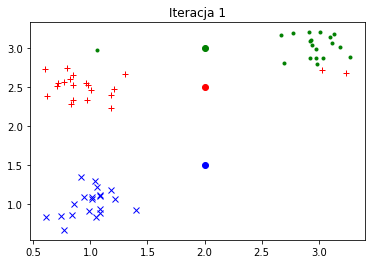
\includegraphics[width=0.6\linewidth]{Rysunki/Rozdzial2/iteracja1.png}
        \caption{Algorytm k-Means: Inicjalizacja algorytmu poprzez losowe rozmieszczenie środków klastrów i wyznaczenie przynależność punktów danych do klastrów}
        \label{fig:kmeans:iteration01}
    \end{figure}

    \begin{figure}[h!]
        \centering
        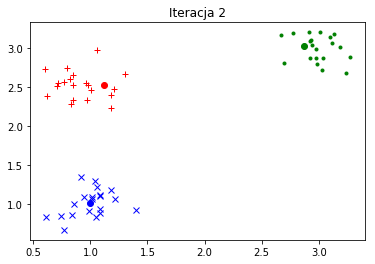
\includegraphics[width=0.6\linewidth]{Rysunki/Rozdzial2/iteracja2.png}
        \caption{Algorytm k-Means: druga iteracja - aktualizacja pozycji środków klastrów oraz ponowne przydzielenie obserwacji do klastrów}
        \label{fig:kmeans:iteration02}
    \end{figure}
    \newpage
    \begin{figure}[h!]
        \centering
        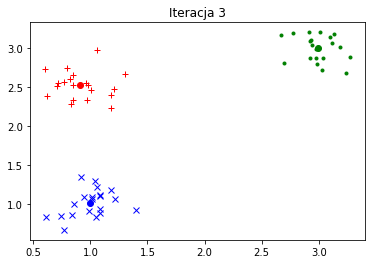
\includegraphics[width=0.6\linewidth]{Rysunki/Rozdzial2/iteracja3.png}
        \caption{k-Means: trzecia iteracja - aktualizacja pozycji środków klastrów}
        \label{fig:kmeans:iteration03}
    \end{figure}
    Głównym problemem algorytmu k-Means jest jego zależność od początkowo wybranych pozycji środków klastrów. Dwa centra mogą znaleźć tą samą grupę i podzielić się obserwacjami, w momencie kiedy dla dwóch środków klastrów przydzieli się punkty danych z tej samej grupy. Kolejne iteracje będą powielały błąd stworzony na samym początku działania algorytmu. Błędne początkowe położenie środków klastrów pokazano na rysunku \ref{fig:kmeans_bad1}.
    \newpage
    \begin{figure}[h!]
        \centering
    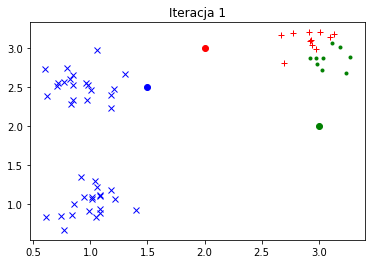
\includegraphics[width=0.6\linewidth]{Rysunki/Rozdzial2/zlaiteracja1.png}
    \caption{Algorytm k-Means: Złe początkowe pozycje środków klastrów}
    \label{fig:kmeans_bad1}
    \end{figure}
    
    \begin{figure}[h!]
        \centering
    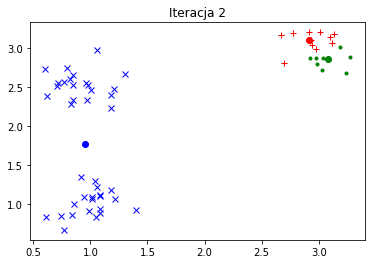
\includegraphics[width=0.6\linewidth]{Rysunki/Rozdzial2/zlaiteracja2.png}
    \caption{Algorytm k-Means: Aktualizacja środków klastrów oraz ponowne przydzielenie punktów danych}
    \label{fig:kmeans_bad2}
    \end{figure}

    k-Means najlepiej radzi sobie z klasteryzacją danych w których, klastry są mniej więcej równej wielkości i mają kolisty kształt.
    \newpage
    
    \subsection{DBSCAN}
    Algorytm DBSCAN (ang. Density Based Spatial Clustering of Application with Noise) jest jednym z algorytmów typu gęstościowego. Został zaprezentowany w 1996 roku przez czterech naukowców: Martin Ester, Hans-Peter Kriegel, Jörg Sander oraz Xiaowei Xu \cite{dbscan}. Działanie algorytmu wymaga podania dwóch parametrów: maksymalnego promienia sąsiedztwa $Eps$ i minimalnej ilości punktów oznaczanej jako $minPts$. Algorytm rozpoczyna działanie od wybrania dowolnego punktu w zbiorze danych. Jeśli w w maksymalnym promieniu sąsiedztwa znajduje się minimalna ilość punktów w odległości od punktu początkowego to znalezione punkty są przydzielane do jednego klastra. 
    
    Algorytm kontynuuje rozbudowywanie klastra do momentu, w którym nie istnieje $minPts$ w obrębie $Eps$ od najbardziej wysuniętego punktu w klastrze.
    
    W przeciwieństwie do algorytmu k-Means, algorytm DBSCAN potrafi dokonać klasteryzacji danych tworzących skupiska o różnych kształtach i wielkościach. Ponadto algorytm potrafi klasteryzować zbiory danych, które zawierają się w innej grupie co ilustruje rysunek \ref{fig:dbscan}
    \begin{figure}[h!]
        \centering
    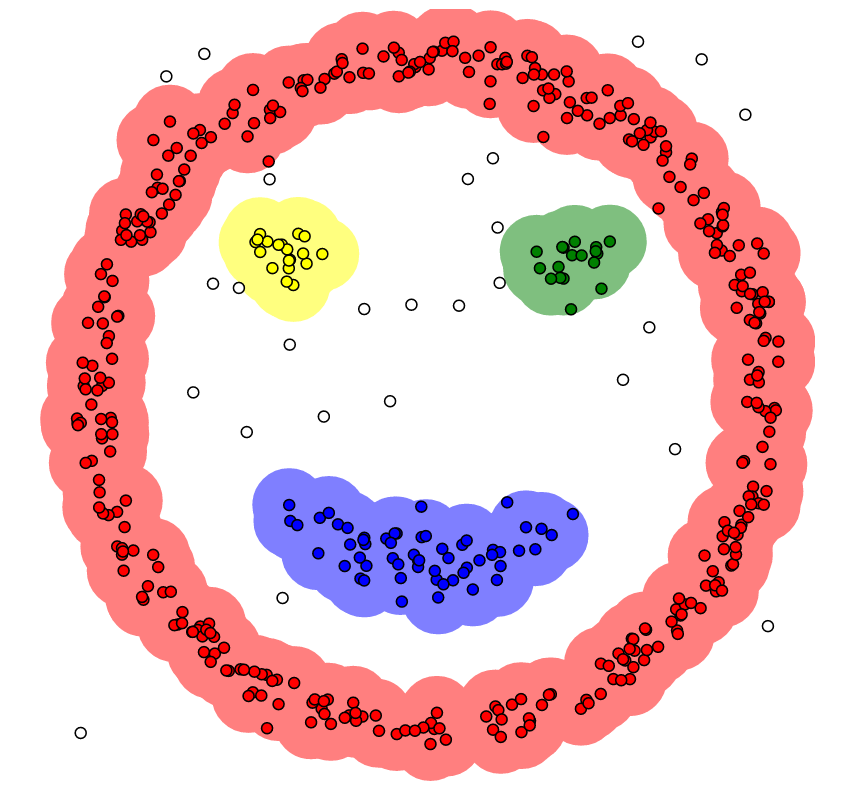
\includegraphics[width=0.6\linewidth]{Rysunki/Rozdzial2/dbscan.png}
    \caption{Przynależność punktów do klastrów w algorytmie DBSCAN}
    \label{fig:dbscan}
    \end{figure}
    
    
\section{Weryfikacja danych}
    \subsection{Histogram} \label{sec:histogram}
    Histogram jest jednym ze sposobów przedstawienia rozkładu empirycznego. Posiada on oś $x$, na której są położone słupki pewnych grup lub cech z danego zbioru danych. Oś $y$ reprezentuje ilość wystąpień danej grupy lub cechy. Histogram można wykorzystać na przykład do prezentacji ilości wystąpień słów we wszystkich dokumentach tekstowych z jednej grupy. Dzięki takiemu przedstawieniu można łatwo określić jaka grupa tych dokumentów posiada jaką tematykę. W niniejszej pracy histogram jest wykorzystywany, aby określić ilość wystąpień klas zwróconych przez algorytm klasteryzacji, względem klas rzeczywistych tych samych dokumentów tekstowych.
    \begin{figure}[h!]
        \centering
    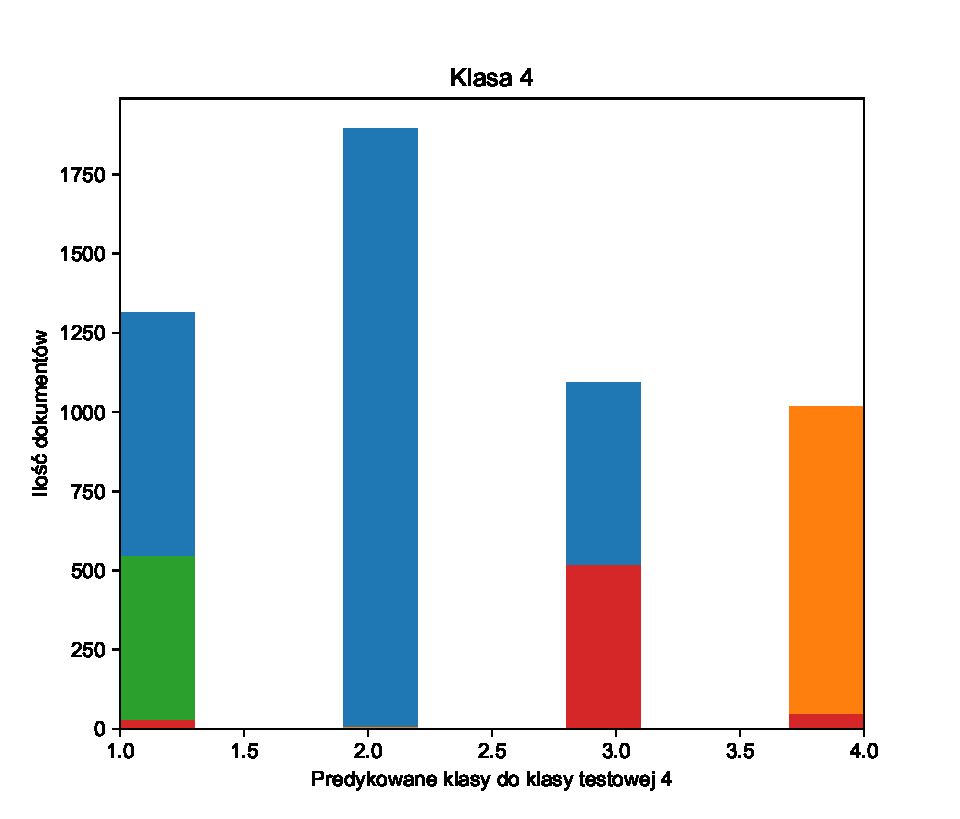
\includegraphics[width=0.7\linewidth]{Rysunki/Rozdzial2/Figure_2.pdf}
    \caption{Przykładowy histogram}
    \label{fig:histogram}
    \end{figure}
    
    \newpage
    
    \subsection{Macierz pomyłek} \label{sec:confusion}
    Macierz pomyłek jest narzędziem stosowanym do oceny jakości wyników z algorytmu klasteryzacji. Na osi $x$ znajdują się etykiety klas, które wyznaczane są przez algorytm klasteryzacji, a na osi $y$ rzeczywiste etykiety klas. 
    \begin{figure}[h!]
        \centering
    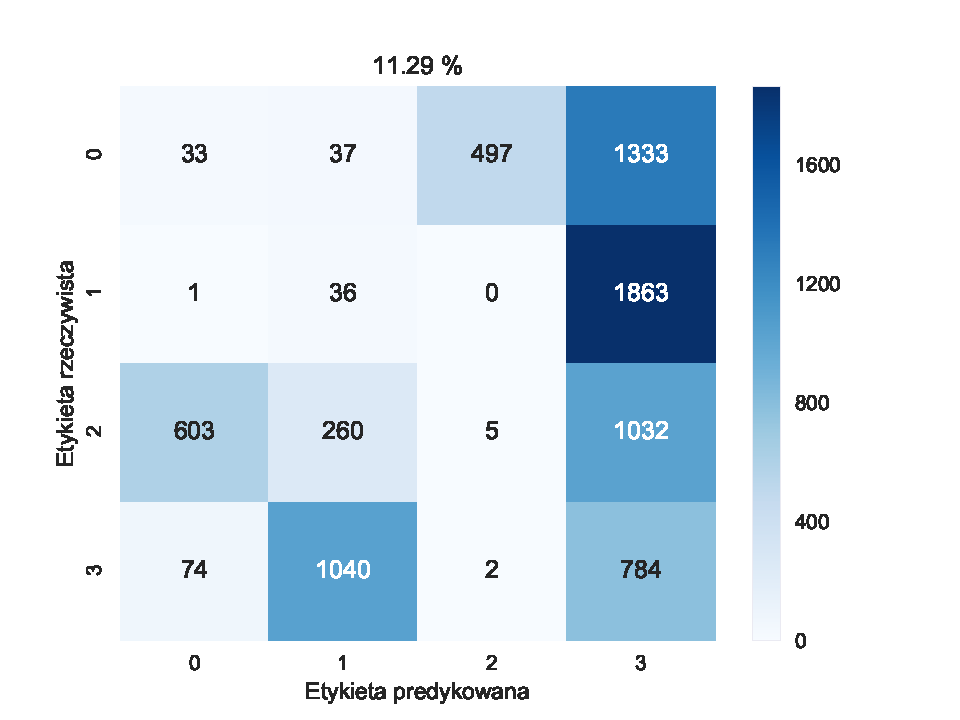
\includegraphics[width=0.7\linewidth]{Rysunki/Rozdzial2/confusion.pdf}
    \caption{Przykładowa macierz pomyłek}
    \label{fig:confugsion}
    \end{figure}
    
    Odczytanie danych z macierzy pomyłek z \ref{fig:confugsion} następuje w taki sposób, że każdy wiersz to klasa rzeczywista analizowanych dokumentów tekstowych. Kolumny oznaczają klasy, które wyznaczył algorytm klasteryzacji. 
    Z macierzy przedstawionej na rysunku \ref{fig:confugsion} możemy odczytać, że dla 33 dokumentów tekstowych mających przypisaną etykietę rzeczywistą "0", algorytm również znalazł oraz przypisał taką samą etykietę.
    
    \newpage
    \subsection{Kombinacje klas predykowanych we wszystkich możliwościach} \label{sec:zamianaKlas}
    Wygenerowanie wszystkich kombinacji przypisań klas predykowanych, pozwoli na znalezienie najlepszego mapowania do klas rzeczywistych. Algorytmy klasteryzacji należą do technik uczenia nienadzorowanego. Z tego względu podczas wielokrotnego uruchamiania algorytmu, pogrupowane dokumenty tekstowe mogą raz znaleźć się w klastrze o etykiecie "1", a innym razem w klastrze "4". By zweryfikować dokładność klasteryzacji potrzebne jest dopasowanie etykiet przypisanych przez algorytm do etykiet rzeczywistych. 
    
    W tym celu stosuje się zamiany klas wygenerowanych przez algorytm w różnych kombinacjach. Schemat działania zamiany klas wygląda w taki sposób, że należy wziąć wyjściową listę etykiet z algorytmu (na \ref{tab:kombinacje} jest to 1 kombinacja), utworzyć macierz pomyłek oraz policzyć trafność przypisania klas (ang. accuracy). Następnie przesunąć każdą predykowaną klasę o jedną klasę w przód, aż do momentu uzyskania początkowych wyników. Dla każdego przypadku liczymy trafność przypisania klas. Wybieramy takie przypisanie, w którym trafność w skali procentowej jest największa.
    \begin{table}[h!]
    \centering
    \caption{Przykładowe kombinacje dla etykiet predykowanych}
    \label{tab:kombinacje}
    \begin{tabular}{|l|l|l|l|}
    \hline
    1 kombinacja & 2 kombinacja & 3 kombinacja & 4 kombinacja \\ \hline
    4           & 1            & 2            & 3            \\ \hline
    4           & 1            & 2            & 3            \\ \hline
    2           & 3            & 4            & 1            \\ \hline
    4           & 1            & 2            & 3            \\ \hline
    1           & 2            & 3            & 4            \\ \hline
    3           & 4            & 1            & 2            \\ \hline
    3           & 4            & 1            & 2            \\ \hline
    2           & 3            & 4            & 1            \\ \hline
    3           & 4            & 1            & 2            \\ \hline
    4           & 1            & 2            & 3            \\ \hline
    \end{tabular}
    \end{table}